\chapter{State of Art}

\section{Technologies}

Many technologies were developed to capture tridimensional information of the environment. In the following section, we aim to describe such systems and describe the basic working principle along with the pros and cons inherent to each ones. These techniques can be categorized into triangulation and time-of-flight.

\subsection{Stereoscopy}

For many years, stereoscopy remain the most popular method for 3D sensing, also because it's working principle resembles our stereoscopic vision. This system uses images taken from a pair of cameras and extract the depth information due to the perspective projection: the position of objects closer differ more than objects farther. To compute depth, features from both images are extracted and correspond together, which makes it a complex and computationally demanding, so it requires fast computers or dedicated software. This system has the advantage of having a good rate of acquisition and having high resolution. Also, color information is available. However, the reconstruction algorithm rely heavy on environment characteristics, like lightning conditions, texture and non-homogeneous regions\cite{klimentjew2010}. This means that this method gives good results for edges and textured areas, but fails to get the depth information of continuous surfaces.

\subsection{Structured Light}

In 2010, the availability of consumer grade depth sensors based on structured light lead to the development of consumer-grade small factor RGB-D cameras, started by Microsoft, with the \textit{Kinect} and followed by other devices, like \textit{ASUS Xtion} and \textit{Intel RealSense}. This cameras come in small form factors, are inexpensive and are capable of capturing both color and depth information at real-time rates\cite{zollhoefer2018}.

This appealing characteristics lead to a huge research and development in 3D reconstruction using this camera, culminating in the KinectFusion algorithm \cite{kinectfusion2011}, capable of a fast and precise 3D reconstruction using a \textit{Kinect} RGB-D camera and commodity GPUs. This algorithm was capable of real-time reconstruction, using a Iterative Closest Point (ICP) for tracking the location of the device and for the registration of new RGB-D data. Nowadays, it is possible to achieve the same result using a phone equipped with a depth camera, like the \textit{Lenovo Phab 2} and with the \textit{Google Tango} software. 

Structured light sensors work by projecting an infrared pattern onto the scene and calculate the depth via the perspective deformation of the pattern due to the different object's depth. This technique, however, yields results far from perfect: the depth values from structured light have significant error or can be missing, specially from objects with darker colors, specular surfaces or small surfaces\cite{shen2013}. 

\subsection{Time of Flight}

Time of flight sensors, or ToF sensors, use the speed of light to measure the distance. A scene is illuminated by a light source and the reflected light is detected back by the sensor. The time that the light has taken to travel back and forth is then measured and the depth is calculated with this time. The measurement dependes on the type of ToF system used, that is ether \textit{continuous} or \textit{pulsed}. In \textit{pulsed} systems, light is emitted in bursts with a fast shutter and the time between the emission and the reception is calculated. \textit{Continuous} systems use a modulated light source and measure the phase-shift between the outgoing and incoming wave.

This technology some advantages comparing to both previous approaches \cite{zollhoefer2018}. First, it is less computationally intensive, because the measurement is directly measured by a specialized sensor. Second, it is partially independent of the lightning conditions because the light detected is emitted by the device itself. Further, it is capable of a dense and accurate depth values, even for continuous or irregular surfaces, unlike the stereoscopic approach. Finaly, tt is much faster that any other method, capable of acquisition rates of hundreds of \si{\hertz}.

However, it has some disadvantages as well. Unlike stereoscopic, which is a passive method, ToF sensors interact with the scene, so are not possible to be implemented in certain environments. Also, the properties of the material, like the reflectivity, color and roughness can have significant effects on the accuracy of ToF sensors. Moreover, multi-path reflections are a common problem of ToF sensors, caused by multiple reflections of the light, causing errors in the measurements. Furthermore, interference can exist if multiple ToF sensors share the same environment. However, it is possible to mitigate this effect.

A popular ToF sensor nowadays is the Photonic-Mixer-Device camera, which looks similarly to a normal image sensor measures the phase shift of incoming light. This sensor is now being used in new generation RGB-D camera, replacing the structured light approach, mainly because it is more resilient to background light, allowing the sensor to work in outdoor environments \cite{zollhoefer2018}. One of this example is the new \textit{Kinetic 2}, that replaced the last depth sensor with this one.

\subsection{LiDAR}

Light Detection and Ranging, or LiDAR, it's one of the most precise and reliable ways to measure distances. It began being used shortly after the Laser invention, in 1960, and it's valuable characteristics lead to the integration of it in the Apollo 15 mission, to serve as an altimeter to map the surface of the moon. Soon after, it was implemented in aircraft to create high-precision and dense earth's surface models. Nowadays, it's applications can be found everywhere where an accurate distance measurement is required, as for example in geology, archeology, geography, oceanography and meteorology.

LiDAR success is related to the use of laser as it's light source. Lasers are capable of emitting beams of light that are monochromatic, narrow and polarized. That is, lasers emit light in a narrow spectrum of light, so they can produce a single color of light, also known as monochromatic light. It improves the resilience against background light, making it possible to use even with sun light. Also, laser photons travel parallel, creating a narrow beam that stays narrow even at large distances, with minimum scattering, therefore measuring the distance in a very small area in the surface. This improves the measurements near sharp transitions, where a bigger area of measurement can cause errors in the measurement. Moreover, laser can transition between an on-off state in a very short time. This is significant to reduce the error of the distance measurement, because it is directly influenced by the time between pulses, and a sharp transition reduces the error in the time measurement. 

The first major application of LiDAR technology was to map and reconstruct the topology of the earth surface. To do it, high range laser scanners are mounted on a plane and are flown above the target area. This is possible due to their high power laser, which allows ranges in the \si{\kilo\meter} range, whiles maintaining precision in the \si{\centi\meter} range. This lasers also have a high sampling rate, in the order of the \si{\kilo\hertz}, which is essencial to maintain a dense sampling, even at high travelling speeds. This high sampling also allows the terrain to be mapped even with high vegetation, because even that only a small percentage of points reach the terrain, there are still a significant number of points. This is just not possible with other methods, like aerial photography. 

Moreover, airborne lidar is also used to detect and classify clouds, which is an important data in meteorology. This is possible by studying the rayleigh scattering effect, which occurs when a laser beam goes through a particles smaller that its wave length, as for example, the water molecules in clouds.  This is essential for modern forecast prediction.

A airborne LiDAR scanner of the Austrian city Retz is shown in \cref{fig:riegl-lidar-scan}, which is available in \cite{potree-retz}, taken with a Riegl laser scanner placed in a Unmanned Aerial Vehicle. \cref{fig:riegl-lidar-scan-big} shows the entire scan with an area of \SI{1300 x 1300}{\meter}, \cref{fig:riegl-lidar-scan-small} shows a portion correspondent to the city, and \cref{fig:riegl-lidar-scan-tiny} shows the town hall, which has an area of about \SI{150 x 70}{\meter}. As can be seen, the result is a massive point cloud that covers a large area while still maintaining a high point density so small details are not smeared out. 

\begin{figure}[p]
    \centering
    \begin{subfigure}{\textwidth}
        \centering
        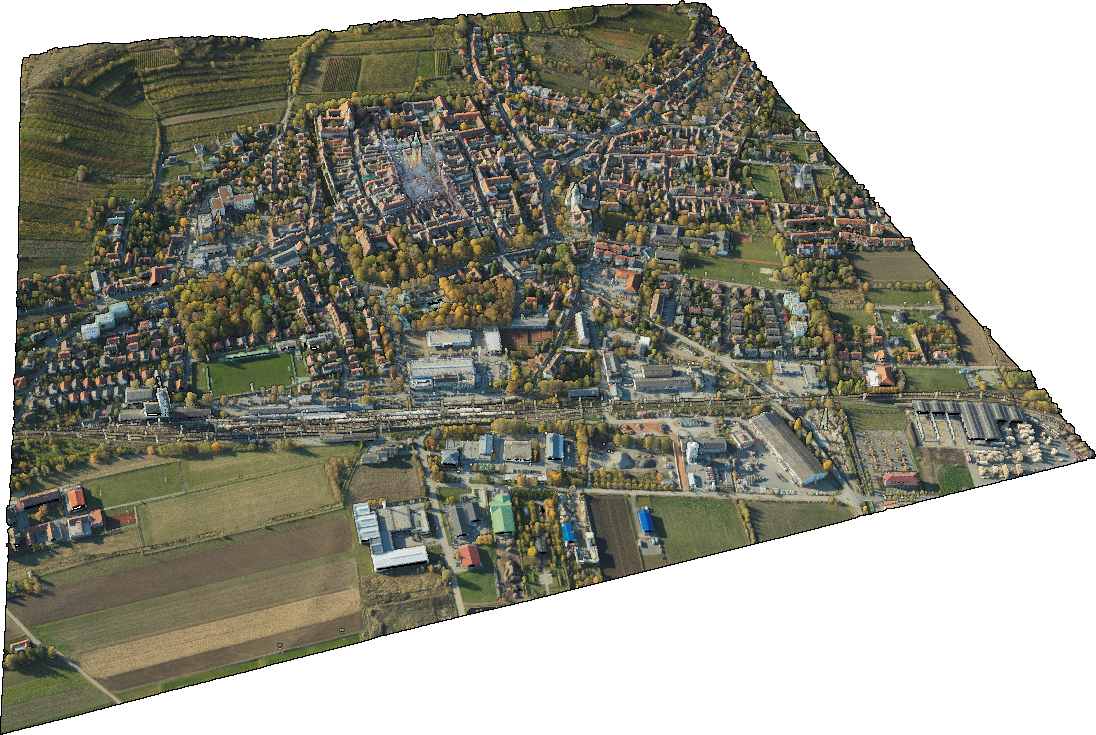
\includegraphics[width=.65\textwidth]{riegel-lidar-scan-big}
        \caption{The entire scan.}
        \label{fig:riegl-lidar-scan-big}
    \end{subfigure}

    \centering
    \begin{subfigure}{\textwidth}
        \centering
        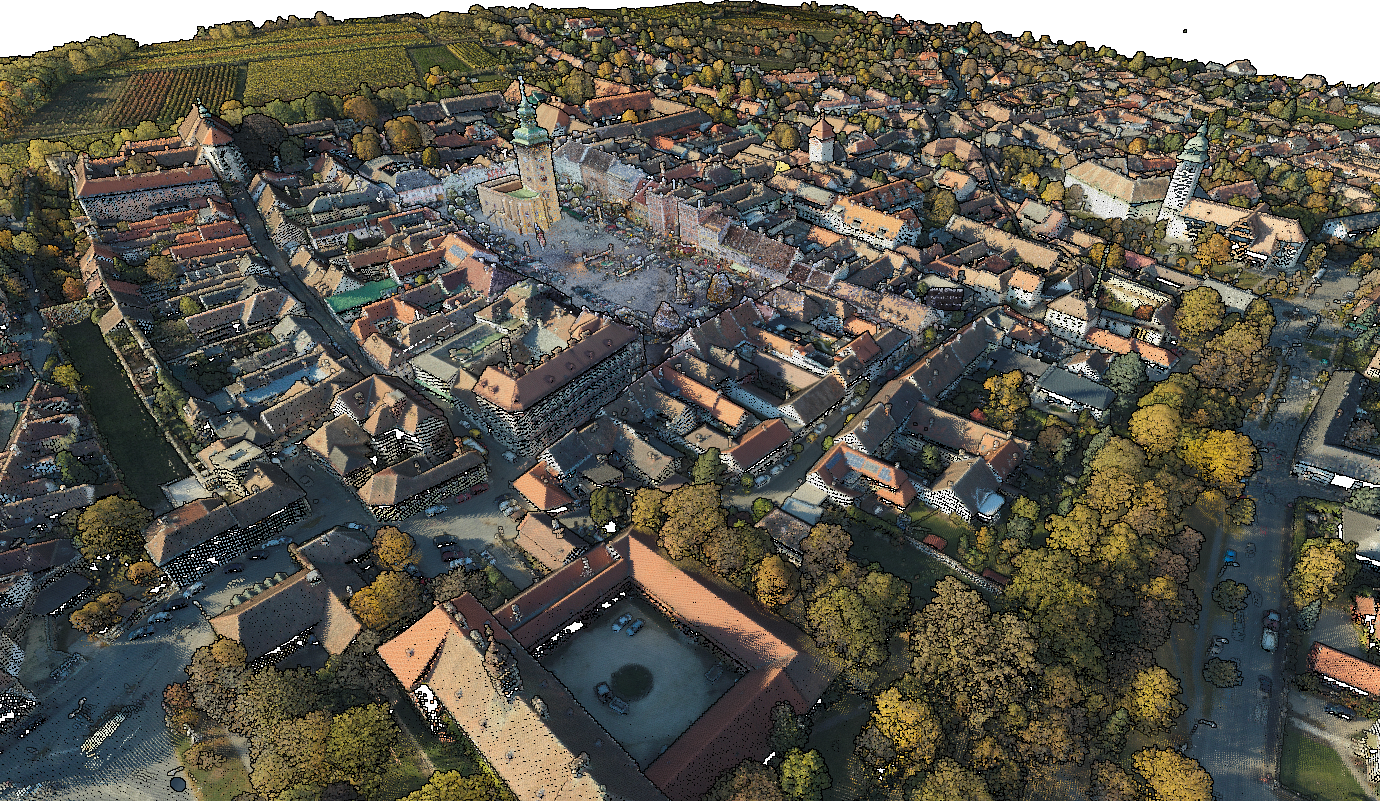
\includegraphics[width=.65\textwidth]{riegel-lidar-scan-small}
        \caption{Pormenor of the City.}
        \label{fig:riegl-lidar-scan-small}
    \end{subfigure}

    \centering
    \begin{subfigure}{\textwidth}
        \centering
        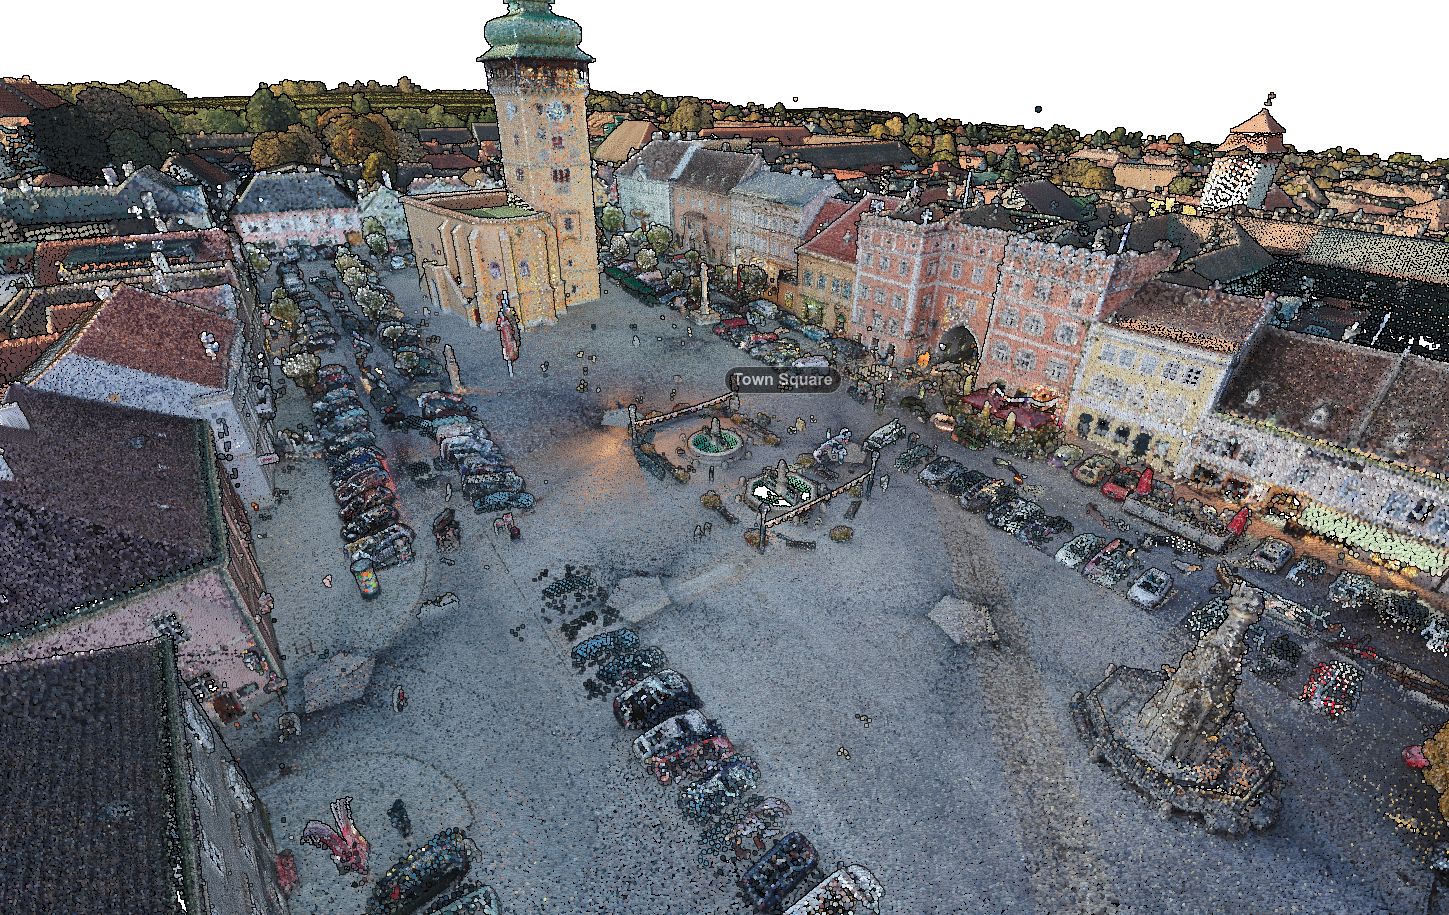
\includegraphics[width=.65\textwidth]{riegel-lidar-scan-tiny}
        \caption{Pormenor of the Town Hall.}
        \label{fig:riegl-lidar-scan-tiny}
    \end{subfigure}

    \caption{Point cloud of Retz obtained by an airborne LiDAR.}
    \label{fig:riegl-lidar-scan}
\end{figure}

In recent years, LiDAR scanner became a fundamental technology for industrial and robotics applications. Their small form factor and high precision are essencial for numerous application. In general, two types of laser scanners exist: the 2D laser scanners and the 3D laser scanners. 

2D laser scanners emit a single laser beam, which is reflected by a rotating mirror to scan across a planar area, as seen on figure X. They are also the most accessible type, as their price ranges range from \SIrange{800}{20000}{\euro}, depending on their characteristics. One example of this laser scanners is the SICK LMS511, shown in \cref{fig:sick-lms511}. 

\begin{figure}
    \centering
    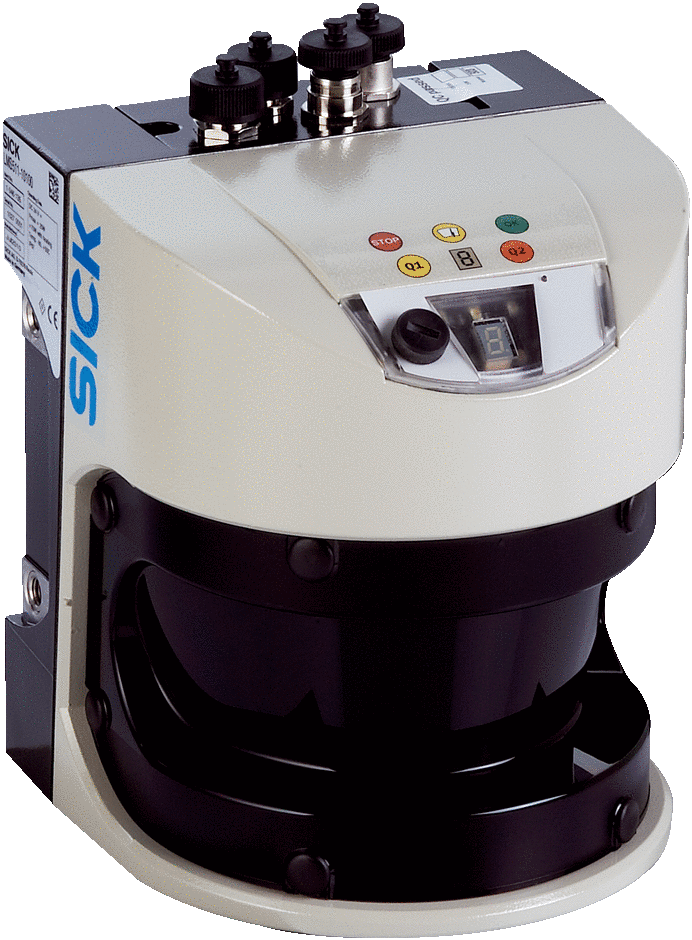
\includegraphics[width=6cm]{lms511}
    \caption{Sick LMS511 2D laser scanner.}
    \label{fig:sick-lms511}
\end{figure}

This laser scanners have a large number of applications. For example, 2D laser scanners are used in autonomous robots, to provide precise 2D mapping information of the environment, which can be user afterwards for location and navigation \cite{siritanawan17}. Compared to other technologies, like stereo vision, this one required small processing power and accurate results, so their application is easy to implement and requires low processing power. 

Another widely used application is intrusion detection. The 2D laser scanner can be spaced in a room or door to detect if any object enters this space. For example, it is used to ensure the safety of workers in industrial environment, ensuring that workers do not get close to working machines. Other example is in theft prevention in museums and banks to secure specific areas against robbery or vandalism \cite{sick-security}.

Recently, 3D laser scanners become available, but at a high price range. One example of this new sensors is the Velodyne, which is a 3D laser scanners priced at \SI{80000}{\euro}. This laser scanners are capable of producing a 3D point cloud directly, unlike the 2D laser scanner. This is possible because they emit multiple laser beams, instead of just one. The laser beams are reflected using a rotating mirror, to get a continuous 3D scan. Moreover, 3D laser scanners are capable of producing a 3D scan at a higher rate than any solution employing a 2D laser scanner. In the case of Velodyne \emph{VLS-128}, shown in \cref{fig:velodyne-vls128}, the number of simultaneous laser beams are \num{128}, with a vertical Field of View of \SIrange{-25}{+15}{\degree} and up to \SI{300}{\meter} range\cite{velodyne-vls128}. This LiDAR laser is capable of a sampling rate of about 9.6 million points per second.

\begin{figure}[h]
    \centering
    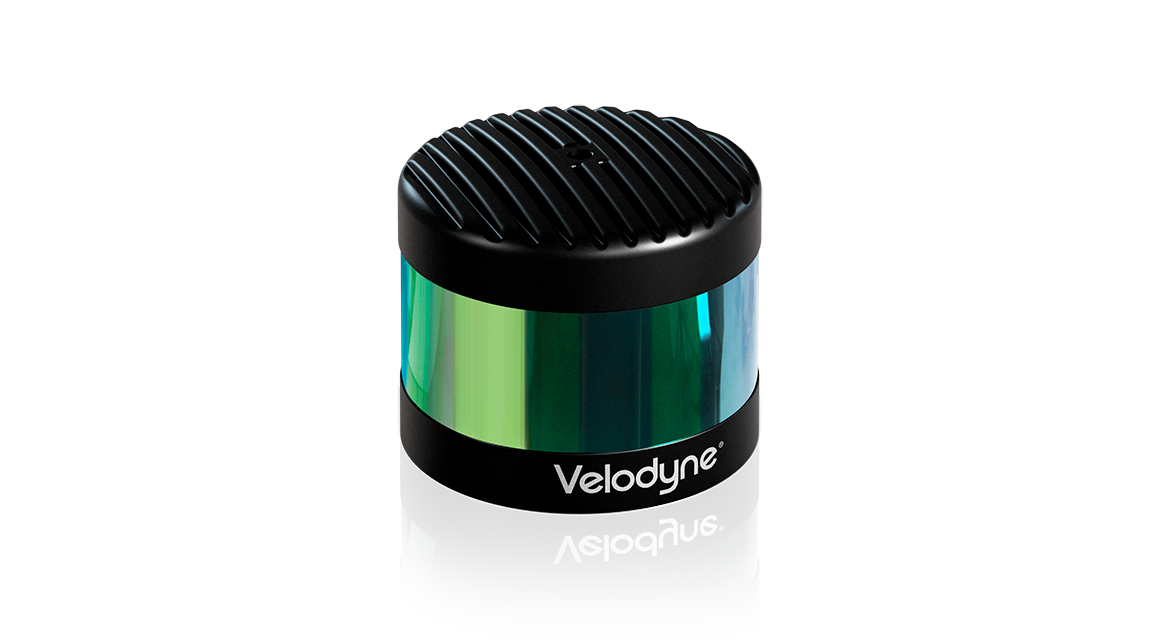
\includegraphics[width=8cm]{velodyne-vls128}
    \caption{Velodyne VLS128 LiDAR laser scanner.}
    \label{fig:velodyne-vls128}
\end{figure}

3D laser scanners are still a very new technology, and are mostly used for high research projects, mainly in autonomous vehicles, like the Google Autonomous car \cite{google-self-driving} or the Stanford Junior Vehicle\cite{montemerlo08}. This application benefits mostly from this scanners high sampling ranges and \SI{360}{\degree} horizontal field of view.

\begin{figure}[h]
    \centering
    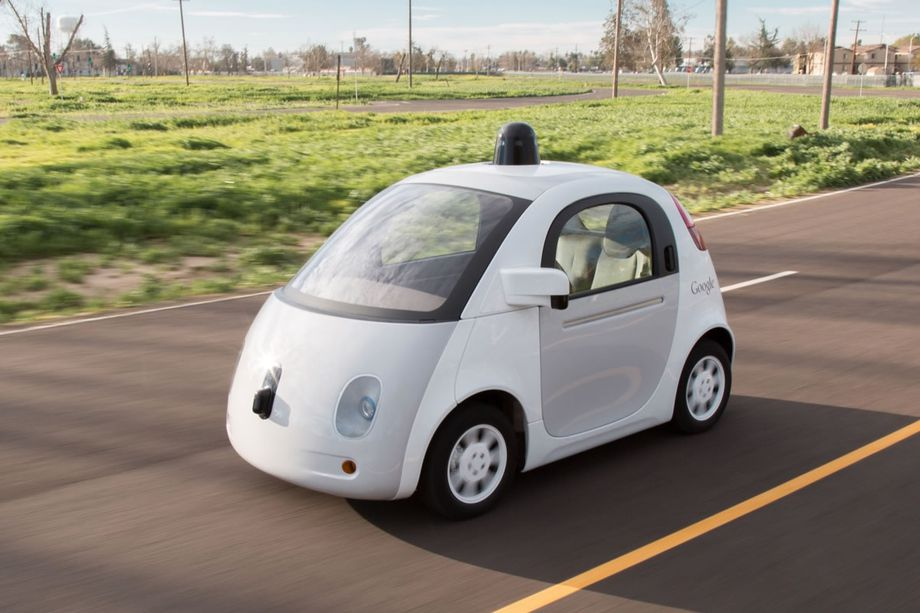
\includegraphics[width=8cm]{google-autonomous-car}
    \caption{Google Autonomous Car.}
    \label{fig:google-autonomous-car}
\end{figure}

\section{Related Academic Work}

Many scientific studies can already be found concerning the research and development of 3D sensors using laser scanners. In most studies, a cheaper alternative using 2D laser scanners is build instead of a more expensive 3D solution. In order to create a full 3D scan, the 2D laser is mounted on top of a moving platform and each individual laser scan is registered on a static frame of reference. The motion of the laser scanner can be classified as continuous or discontinuous. Usually a continuous motion is used for real-time systems, like autonomous vehicles, while a discontinuous motion is used when real-time is not important, like accurate 3D reconstructions of scenes. In the following paragraphs we describe such systems that were developed so far.

In \cite{surmann2003}, a mobile robot was capable of autonomous navigation, thanks to a tilting \textit{LMS200} laser scanner, that provided a depth map of the front of the robot, with a maximum resolution of $721\times256$ points. However, a scan of $181\times256$ took about \SI{3.4}{\second}, and scans with more points ($361$ or $721$) meant double or quadruple this time, making it not suitable for real-time operation. This previous system had a limited field of view, so in \cite{zcai05} a \textit{LMS291} was mounted on a pan-tilt unit for generating a 3D point cloud with a parameterized field of view.

More recently, 3D laser scanner began being developed for continuous operation for real-time for Simultaneous Mapping and Navigation, or SLAM, for autonomous robots. This was specially due to the \textit{DARPA Grand Challenge}, that offered a \$1 million cash prize to the fastest autonomous unmanned vehicle that completed a 300 miles track. In \cite{maurelli2009}, a 3D laser scanner (\cref{fig:maurelli-laser-scanner}) was developed by placing two \textit{LMS200} planar laser scanners on a rotating vertical axis, capable of generating a high-quality 3D point cloud with a \SI{360}{\degree} field of view. Lots of other lasers were developed by rotating the laser in a continuous motion using a turntable \cite{nemoto2007}, a swinging platform \cite{yoshida11}. This sensor also became lighter, compact and modular, making it possible to integrate in multiple systems easily. One of this systems is \textit{KaRoLa} (\cref{fig:karola}), described in \cite{karola14}. This laser scanner was then applied to several system, specially in search and rescue robots.

\begin{figure}[h]
    \centering
    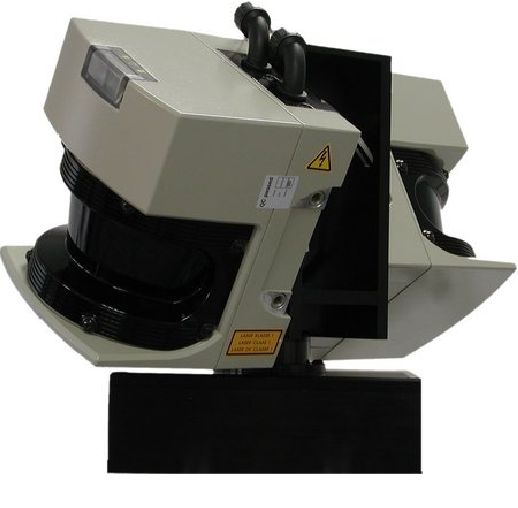
\includegraphics[width=5cm]{maurelli-laser}
    \caption{3D laser scanner developed in \cite{maurelli2009}.}
    \label{fig:maurelli-laser-scanner}
\end{figure}

\begin{figure}[h]
    \centering
    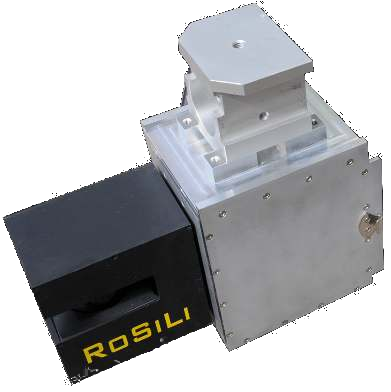
\includegraphics[width=5cm]{karola}
    \caption{The KaRoLa 3D laser scanner.}
    \label{fig:karola}
\end{figure}

The 3D laser sensors are only able to reconstruct the geometry of the scene. Some sensors are also able to measure the intensity of the reflected light, create a grayscale value for each point. This intensity is measured, of course, in the frequency spectrum of the emitted light of the sensor, which is usually infrared (\SI{950}{\nano\meter}). To reconstruct the color, one or more cameras are coupled to the sensor, and both depth and color data is merged, in a process called fusion, to create colorized model. This is specially important for area like architecture or archeology, where color information is very important. Such work can be seen on \cite{pdias2006}, where a 3D sensor like the one described in \cite{surmann2003} was paired with a camera, to generate a 3D reconstruction with color. Another technique was created in \cite{stamus2000}, where the range and color images are captured separately and then a method is used to make the registration of the color images in respect to the extracted geometry. The registration was optimized for scenes with high geometry content.

This techniques are applied, for example, in cultural heritage, to model important art pieces. One of the most famous examples is the Michelangelo project \cite{levoy2000}, which developed a technique to register data from a triangulation sensor and color image data to reconstruct the 3D geometry of the statue of Michelangelo's David. One of the challenges in this project was to capture the chisel marks in the surface of the status, requiring a resolution of \nicefrac{1}{4} \si{\milli\meter}, in a statue \SI{5}{\meter} tall~\cite{levoy2000}.

\section{Comercial Solutions}

In this section two commercial solutions are shown and discussed. Both solution aim for a precise 3D reconstruction with color information, but the first solution does it with a structured light sensor and the second solution relies on a laser scanner. 

\subsection{Matterport}

\emph{Matterport} is advertized as a all-in-one solution, capable of both 3D reconstruction and capture 4K resolution images from the scene. Their target are mostly the reconstruction of indoor scenes, more specifically, the interior of houses. Then, the 3D model can be used to showcase the interior of the house, using both virtual reality or panoramic photography, or to make 3D measurements and automatically generate floor plans\cite{matterport}.

\emph{Matterport} offers two products: a 3D camera and a cloud service to process the raw data taken with the camera. The camera, as seen in \cref{fig:matterport-camera}, consists of two sensors: a structured light sensor and a photographic camera\cite{matterport}. The structured light sensor has an advertized accuracy of $99\%$ within the \SI{4.5}{\meter} maximum range. The Photography sensor is a 4K HDR camera.

\begin{figure}[h]
    
    \centering
    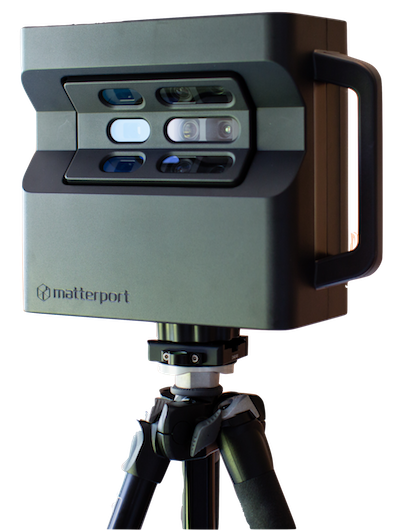
\includegraphics[width=5cm]{matterport}

    \caption{Matterport Pro2 Camera.}
    \label{fig:matterport-camera}

\end{figure}

The overall process to capture a scene is fast and easy: the 3D camera is placed on a tripod and is controlled remotely. Each acquisition takes about \SI{20}{\second} and the result is a 3D colorized mesh with 4 million vertices and a \SI{360}{\degree} panoramic photography with 134.2 MP. To scan an entire environment, an operator moves the camera to each space and make multiple new acquisitions from that space.

A set of models reconstructed from the with the Matterport solution can be found in \cite{matterport-gallery}. As an example, the model named "Pennsylvania Craftsman Home" \cite{matterport-house} can be seen in \cref{fig:matterport-model}. This model represents the complete interior of an house and looks very realistic.

\begin{figure}[h]
    
    \centering
    \begin{subfigure}{\textwidth}
        \centering
        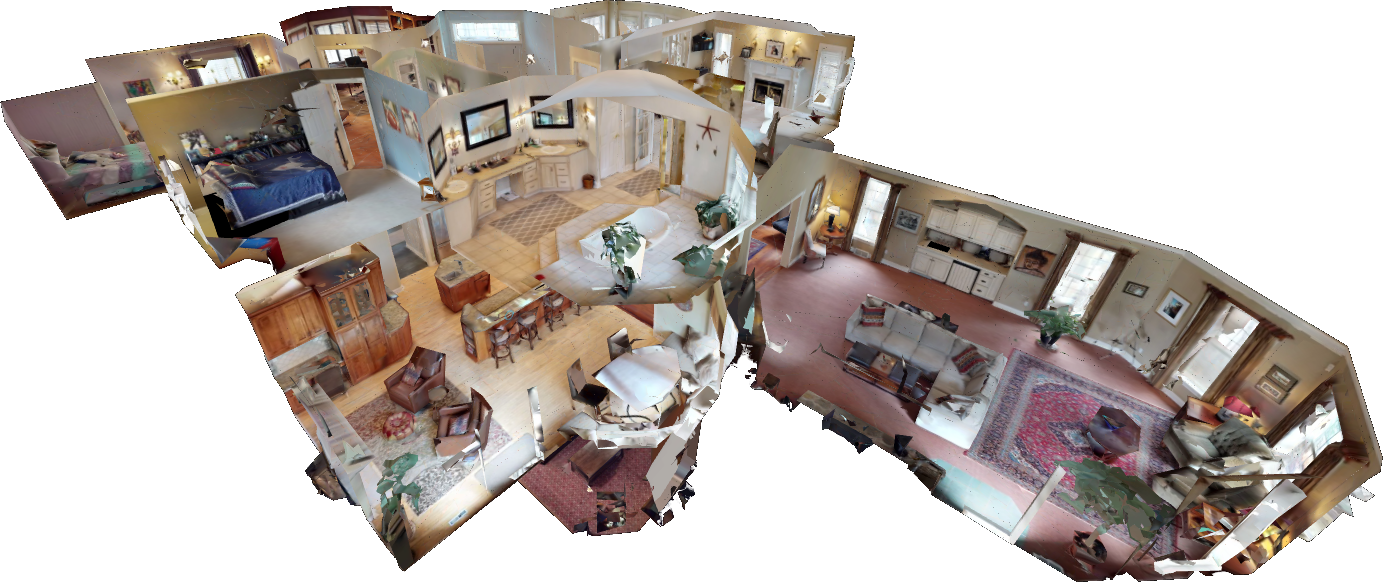
\includegraphics[width=10cm]{matterport-scan-side}
        \caption{Side view.}
    \end{subfigure}

    \begin{subfigure}{\textwidth}
        \centering
        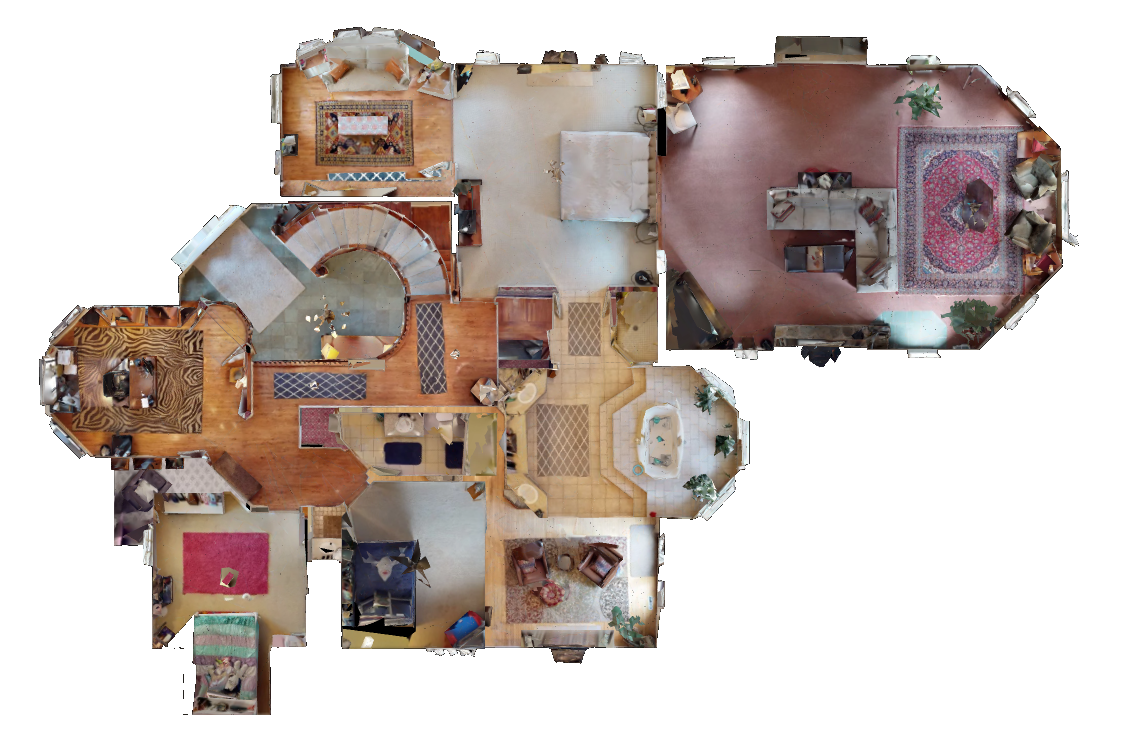
\includegraphics[width=10cm]{matterport-scan-top}
        \caption{Top view.}
    \end{subfigure}

    \caption{Matterport "Pennsylvania Craftsman Home" model.}
    \label{fig:matterport-model}
\end{figure}

\subsection{Faro Focus}

Faro Focus \cite{faro-focus} are a series of 3D laser scanners targeted for the sectors of architecture, engineering, construction and product design. As such, this solution is capable of fast 3D reconstructions both on outside and inside environments with great accuracy. The 3D scanner, as seen in , is design for portability and is equipped with a laser scanner with a precision of \SI{+-1}{\milli\meter} and a range of \SIrange{0.6}{350}{\meter}, and a 8 MP HDR camera.

\begin{figure}[h]
    \centering
    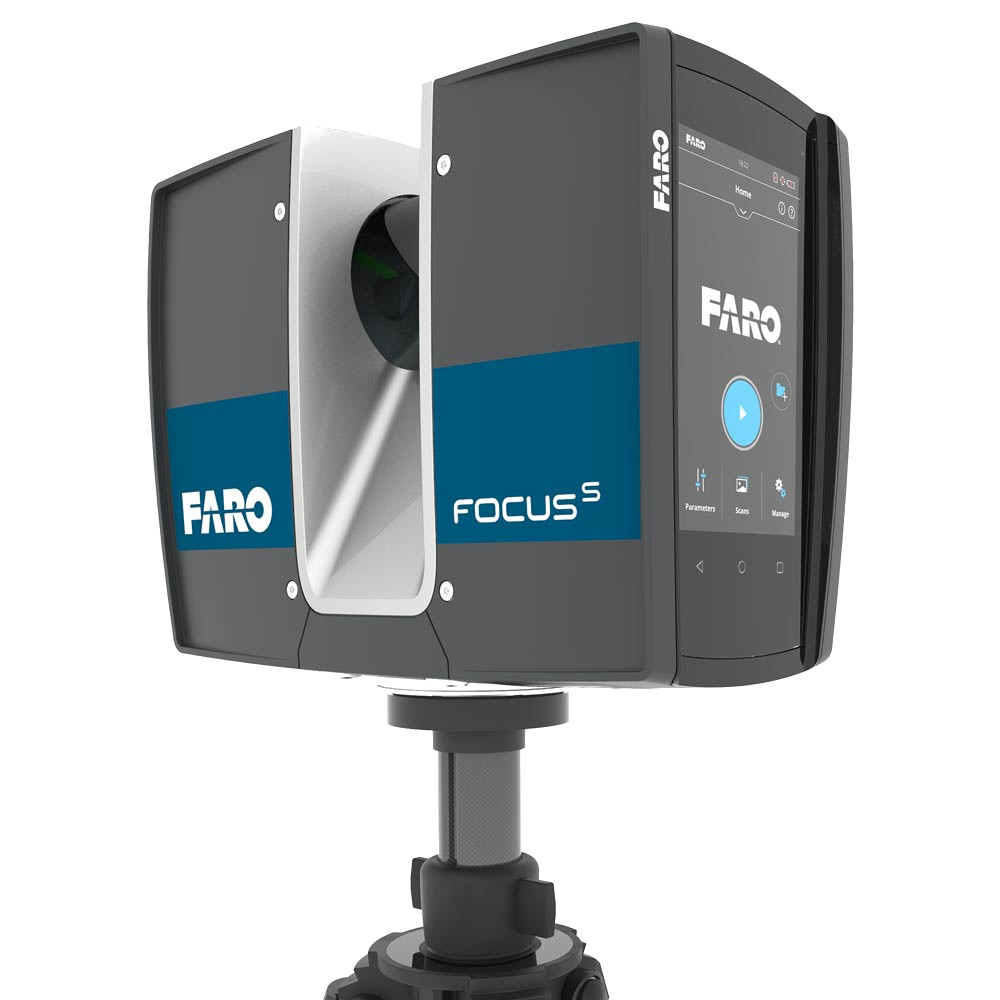
\includegraphics[width=6cm]{faro-focus}
    \caption{Faro Focus 3D laser scanner.}
    \label{fig:faro-focus}
\end{figure}

An acquisition, like in the \emph{Matterport Pro2 Camera}, is quick and easy, but does not require any remote computer, as the scanner incorporates a touch LCD screen. All the subsequent processing is done afterwards in a computer, using their proprietary software.

Faro Focus scans are very precise, as they are used for precise measurements of the reconstructed scene. As an example, a scan obtained by the Faro Focus can be seen in \cref{fig:faro-scan} (from \cite{faro-scan}).

\begin{figure}[h]
    \centering
    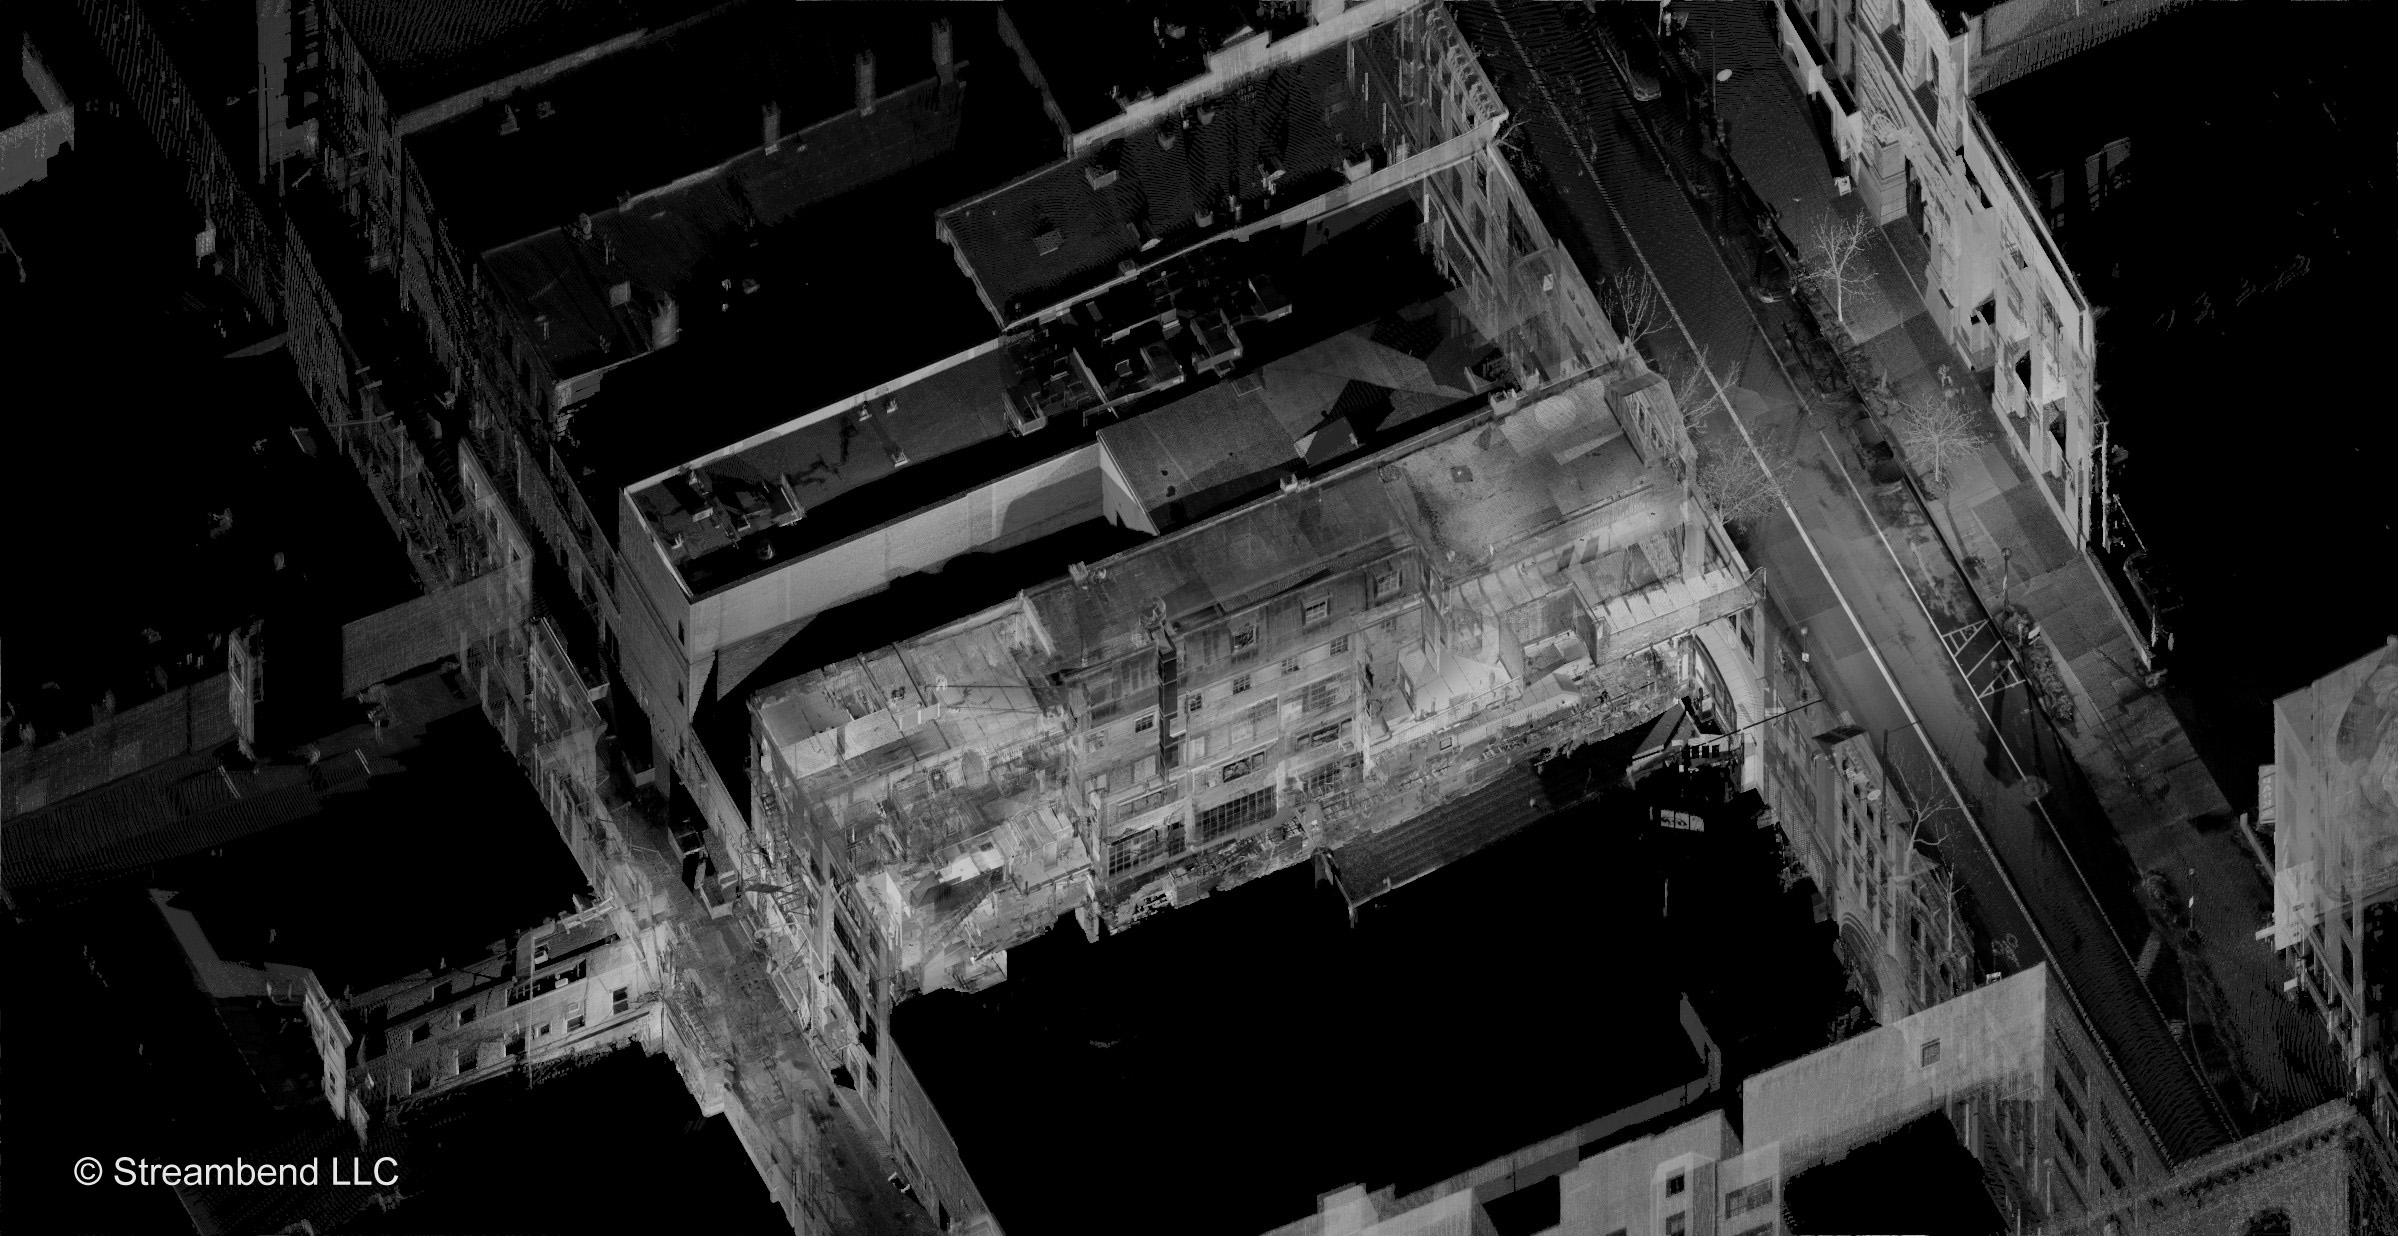
\includegraphics[width=12cm]{faro-scan}
    \caption{Faro 3D scan.}
    \label{fig:faro-scan}
    
\end{figure}

\section{3D Digital Models}

Recreating a real scene with computer graphics is an important topic in today's world and many advancements are being made to create the illusion, for the user, that what he is seeing is real. Many technologies and advancements appeared, like Virtual-Reality, high definition models, photo-realistic rendering and dynamic models. One of the biggest objectives of 3D reconstruction is the possibility of using this technologies to recreate real 3D scenes, making it possible for anyone with a computer or a VR-set to experience this scenes. The number of applications are huge, but the problem remains: how can we save a 3D environment?

In computer graphics, the most common representation is a polygonal mesh. It is composed by a collection of vertices, edges and faces composing a polygon that represents a simplification of the original geometry. Because of it's flexibility and wide use, graphic cards are specially optimized to render this meshes and the result are very good. Properties of the object, like color and material, can be added per-vertex or per-face, making it a flexible model to save all the details of the scene. There are also many drawbacks to this representation, for example, the inadequate representation of non-linear surfaces, requiring large sampling to represent it reliably.

However, it is impossible to get a mesh directly from a 3D scanner, so a simpler model is used instead: the point cloud. A point cloud is a set of points sampled from the surface of the objects, so it's detail depend largely on the density of the points. Point clouds can also store extra data pixel-wise, for example, color, normals, intensity or segmentation index.

Because it's such a simple representation, it is very used in robotics and 3D vision, for example, in search and rescue robots, for mapping and navigation, in unmanned vehicles, for road segmentation and in bin-picking robots, for object segmentation. However, it is not adequate for scene reconstruction, because a realistic model requires a huge density of points, which is unfeasible for numerous reasons. To start with, rendering point clouds is slow in modern graphic cards, because the rendering pipeline is not optimized for it, resulting in slow framerate, which then causes a poor experience for the user and unsuitable for VR. Despite new advancements in point-rendering algorithms, capable of rendering point clouds with billion points in commodity hardware \cite{wimmer2006}, it will always be a limiting factor for this model. Also, some of the processing algorithms for point clouds have non-linear time complexity, so point clouds with many points can have long processing times. One of the most wide-spread solutions is to down-sample the point cloud to speed up the algorithms. Finally, large amounts of data are repeated in the point cloud, resulting in redundancy problems and large file sizes. For example, planar surfaces require the same density of points as any complex surface, while in meshes, the density of faces can be adjusted to the gradient of the surface.

This problems are usually solved by performing a triangulation of the point cloud, a process where a mesh is produced, therefore solving all the problems inherent to the simplistic point cloud model. However, this process requires a fine point cloud, that usually require many man-hours of thorough processing, to yield acceptable results. That is why LiDAR Laser scanner are so valuable for 3D reconstruction, as it yields raw point clouds with a better definition than any other technology, requiring less post-processing work in the triangulation process.
